%Service Oriented Computing
\section{Service Oriented Computing}
\label{ServiceOrientedComputing}
%--- Brief overview on SOC and SOA

\subsection{Services and composition, SOC and SOA}
\label{SOC&SOA}
During the years preceding the large spread of the Internet, companies used to create their own software systems, in order to obtain highly customized and specific services, rarely focused on the accessibility by external partners.
Today, with the necessity of exchanging information among different companies and businesses, and the push made by the large growth of the Internet, the focus has moved to the integration and the coordination of the existing softwares, namely, the integration of these systems over larger networks.
Defining a \textit{service} as a distributed application that exports a view of its functionalities  \cite{DiLorenzo08}, what is needed is the possibility to compose different services together.
For example, it might be useful to integrate a service (already available on a net), providing maps of a city's streets, with a web-based service listings telephone numbers of a given city zone, resulting in a new service showing telephone numbers on the map. %\fxnote{I might add a picture to better show the example here} FIXME
  
The \textit{Service Oriented Computing} (SOC) is the paradigm that attempts to wrap and adapt existing applications into new services, which should comply to three main requirements \cite{DiLorenzo08,Papazoglou03}:
\begin{itemize}
 \item technological independent: the service should be accessible via well known protocols and have a descriptions available on most of the IT environments.
 \item loosely coupled: the client and the provider of the service should not know each other's internal details.
 \item location transparent: clients should be able to get information and access to a service, irrespectively of their location. 
\end{itemize}
Eventually the SOC paradigm makes use of services as the atomic components for developing new applications (which, in turn, can be services too \cite{Papazoglou03}.


To apply the SOC paradigm, there is a need of an architecture infrastructure style, which gives the directives and guidelines to build such a service.  
The architectural infrastructure of the SOC is called \textit{Service Oriented Architecture} (SOA). 
The idea behind the SOA is to describe, publish and make available services (generally speaking, a combination of services) obtained from a preexistent set of applications. 
To achieve the results of making non-homogeneous applications, using different technologies and running on different platforms, work together, SOA makes use of standard interfaces and messaging protocols. This way each of the applications become an atomic, well defined and ready to be connected component. 
The SOA presents an architecture devised in three main components \cite{Pernici04} as shown in Fig. \ref{fig:The Service Oriented Architecture (SOA)}:
a \textit{service provider}, which makes the service available. The service provider registers its service to the \textit{service registry}, which contains the list of available services and their descriptions. After the registration, the service provider waits for a client to request a service. The service registry can also apply custom access control policies or be entirely public. 
The \textit{service client} contacts the service registry to \textit{find} a service, it gets a contract and the address of the service, making a so called \textit{bind} with the provider. Then it \textit{uses} the service.


Being the realization of services usually based on the reuse of previously existent software, there are many ways to realize it and they can also be combined. For a company, the realization can go from the complete in-house realization to the outsourcing, to buy/leasing just parts of the needed services or to using wrappers/adapters to reuse the legacy software.
To conclude, from the SOA point of view, services are like black boxes, they can be invoked by service clients independently, without the need of knowing internal details. This makes clients and providers logically decoupled, the client only needs to know the name, the interface and the version of the service. Of course, provider, client and register must be able to use a common communication channel. 

\subsection{Web Services}
\label{WebServices}
We have seen that SOA is an architecture style aimed at the creation of services but it does not address the communication medium. \textit{Web Services} (WS) are an instance of a SOA where the communication channel is the web \cite{Pernici04}.
Web services implement the SOA through the application of three main technologies: \textit{SOAP}(Simple Object Access Protocol), \textit{WSDL}(Web Services Description Language) and \textit{UDDI}(Universal Description, Discovery and Integration).
On the picture of the SOA showed above, we can add these three components, as shown in Fig: \ref{fig:SOA with webServ implement.}. The SOAP is the web protocol used to exchange messages among the parties. WSDL is the language used by the service provider to fully describe the offered service. At last, UDDI is used by the service registry to make a service easy to find, abstract its technology and make it accessible to the clients.
In the next paragraphs we have a brief look into these three technologies.

\subsubsection{WSDL (Web Services Description Language) }
WSDL is a language based on \textit{XML}(eXtensible Markup Language) and it permits to unambiguously describe a web service. For example, it can describe the input parameters a client must provide to use the service and the type of the result the client should expect. 
A WSDL description starts with a \textit{service} tag that identifies a group of related services. Each of the services is then described as following.
The first element is the \verb|port| which identifies the address and the protocol to access the service (e.g. from the IBM online examples,\cite{IBMWSDL} \\
\verb|<soap:address location="http://www.snowbo.../EndorsementSearch"/>|). \\
With \verb|portType|, there are given the specifics of any \verb|operation| that can be used by the client, for example, the input/output parameters or the error messages. The \verb|operation|s comply to one of 4 main patterns: the \verb|One_way| (client sending a message to the provider), the \verb|Request_response| (client sending a message and waiting for an answer form the provider), the \verb|Solicit_response| (Provider sending a message to the client and waiting for a response) and the \verb|Notification| (provider sending a message to the client).
The elements to define the messages and the types used by the service are \verb|message| and \verb|types|. The first specifies the structure of a message to be exchanged. The second, is used to define the atomic types (integer, string, etc.) or new custom types. 
The most important elements in a WSDL service description are summarized in Table \ref{tab:WSDLElements}.

Eventually, we can see that WSDL proposes a static picture of the service. It defines the address and the way to access the service, the operations and, for each of them, the input/output elements to be provided, but it has no notion of the order in which the operations should be called. For example, to access an online shop service, there might be the need to first perform a login operation, check the item availability and last, buy the item. Such a order or workflow, though, it is not addressed in a WSDL description. This workflow represents the dynamic behavior of a service and it is addressed by the \textit{WorkFlow Management Systems} (WfMS), discussed in the following section.


% - Who is going to deal with the logic and flow of the composition? \nl 
% - Two main approaches: Orchestration and Choreography, where is the difference \cite{Peltz03} \nl
% - The concept of Workflow management \cite{Aalst98} (picture) and why BPEL is good at it.  \nl
% 
%%%%%%%%%%%%% WSDL TABLE of characteristics %%%%%%%%%%%%%%%%%%%%%%%%%%%%%%%%%%%%%%%%%%%%%%%%%%
\begin{table}
\begin{center}
\begin{tabular}{l p{11cm}}

						\toprule
						\addlinespace[0.2cm]
\textbf{WSDL element} 	& \textbf{Description}	\\ 
						\cmidrule(l){1-2}
\verb|port| 		& It identifies the address where the service is found and the protocol to access it 				\\[0,1cm]
\verb|portType| 	& It provides the description of the service, using the \textit{operation} element 				\\[0,1cm]
\verb|operation| 	& It is a basic functionality provided by the service. It lists the input and output messages that are exchanged, in one of the four communication patterns 														\\[0,1cm]
\verb|message| 		& It specifies the format of messages to be exchanged, e.g. the name and type of the variables they contain 	\\[0,1cm]
\verb|types|		& The atomic or user-defined data types in use  								\\[0,1cm]
\verb|binding|		& Given a portType, it describes how this is implemented in the specific protocol 				\\[0,1cm]
	 
						\addlinespace[0.2cm]
						\bottomrule
\end{tabular}
\end{center}
\caption{Basic WSDL elements and their description}
\label{tab:WSDLElements}
\end{table}
%%%%%%%%%%%%%%%%%%%%%%%%%%%%%%%%%%%%%%%%%%%%%%%%%%%%%%%%%%%%%%%%%%%%%%%%%%%%%%%%%%%%%%%%%%%%%%

\subsection{Wf management: Orchestration vs Choreography}
\label{WFManagement}
%This workflow is the dynamic behavior of a service and it is addressed by the \textit{WorkFlow Management Systems} (WfMS), discussed in the following section.
The workflow description, needed to address the behavior of a web-service is controlled by the \textit{WorkFlow Management Systems} (WfMS). The activities are performed following an execution flow based on four main patterns \cite{Pernici04}: \verb|sequence|, \verb|AND_split|, \verb|OR_split|, \verb|join|. These patterns permit to create generic workflows which are scheduled depending on the availability of the resources.
Two approaches for the workflow management exist: Orchestration and Choreography \cite{Peltz03}. Although the two approaches might overlap, their aims differ (see Fig. \ref{fig:OrchAndChor}). 

\paragraph{Orchestration}
Orchestration describes the realization of an executable business where the overall control is given to one party. For example, we can show how a travel planner web service works (see Fig. \ref{fig:orchestration}). Once a client sets the dates and destination of his travel, the travel planner service (coordinator) contacts other three services to book a flight, a hotel and a car. The requests and responses to and from the orchestrated services, are dealt by the coordinator, which takes care of reporting the found travel information back to the client.
These three services can be separated modules, belonging to different companies and implemented with different technologies.
\paragraph{Choreography}
Choreography also describes the realization of an executable business process, but there is no party having overall control. Here each party collaborates and provides its part and role for the final result. Using the previous example (see Fig. \ref{fig:choreography}), we can notice that the stand alone services have no coordinator. They collaborate exchanging messages among each other. Eventually, choreography, takes care of the interactions among the services more than executing a process from one party's perspective.

\subsubsection{Workflow Management for Web Services}
Among the workflow management systems, there are: FIXME Introduce BPEL and describe it in the next subsection.


%%%%%%%%%%%%%%%%%FIGURE %%%%%%%%%%%%%%%%%%%%%%%%%%%%%%%%%%55 
 \begin{figure}
\centering
\subfigure[Service orchestration. The travel planner service coordinates the activities of the car rental, flight booking and hotel booking services. ]{
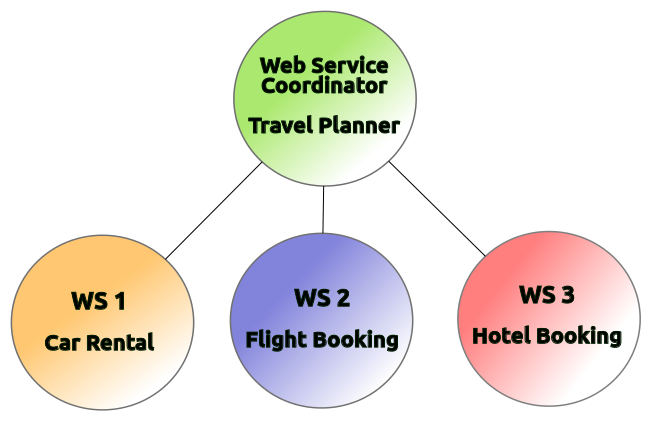
\includegraphics[scale=0.32]{pictures/FigOrchestration}
\label{fig:orchestration}
}
\hspace{2mm}
\subfigure[Service choreography. The services here collaborate to realize the main objective.]{
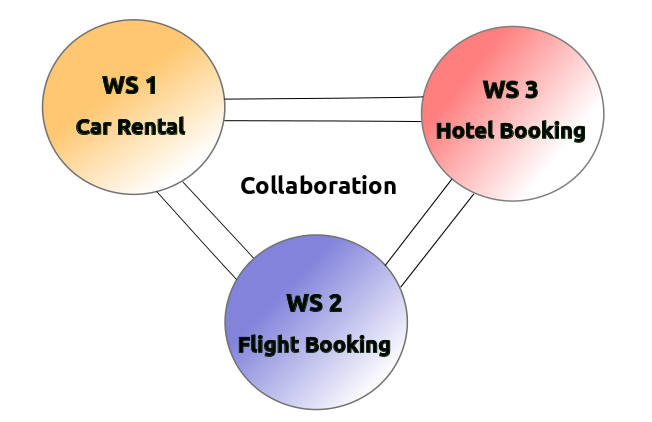
\includegraphics[scale=0.32]{pictures/FigChoreography}
\label{fig:choreography}
}
\caption{Example of service orchestration versus service choreography}
\label{fig:OrchAndChor}
\end{figure} 
%%%%%%%%%%%%%%%%%%%%%%%%%%%%%%%%%%%%%%%%%%%%%%%%%%%%%%%%%%%%%%%

\subsection{BPEL}
\subsection{Java RMI}
- Overview, features. - Why? it can run everywhere, lightweight scenarios.
%\subsection{Jet}
%\subsection{EMF and Open Architecture Ware (Eclipse)}
%\subsection{other...} 


% %---Where the problem is---
% \subsection{BPEL, its drawbacks and the use of WSs in a lightweight scenario}
% %\subsection{The drawbacks of using BPEL (BPEL and its possible drawbacks)}
% - BPEL, the de-facto standard concerning web services composition. \nl
% - Overview and brief review\nl
% - What do we use of it, the whole language or just a part? \nl %Questo dove andrà??
% - Problems: It works over Distributed Systems, engine powerful but heavy, DS not always available. \nl %i problemi che ha in generale e quelli specifici al nostro caso
% 
% %---Why we face the problem and which is the possible solution (and aim of the work)---
% %\subsection{Web Services Composition in lightweight scenario}
% - That's our question \nl
% - Sometimes we might need services composition working in less powerful environments than distributed systems. Examples? \nl
% - But we don't want to create a new application from scratch neither...(change hardware?).  \nl



